% AR/ar_section.tex
% Univariate AR family (RW, AR(1)-YoY, AR_lags, AR+_lags, AR_ranks) on Japan CPI.
% Designed to be \input{} from a parent document. Requires:
%   \usepackage{amsmath, amssymb, booktabs, graphicx}
%   \usepackage{threeparttable}   % for \begin{tablenotes} in horizon_table.tex
% Paths assume the parent document is compiled from the project root; adjust
% the \graphicspath / \input prefixes if compiled elsewhere.

\subsection{Univariate AR\textsubscript{ranks} on Japanese Headline CPI}
\label{subsec:ar_ranks_japan}

\paragraph{Setup.}
Following the AR\textsubscript{ranks} construction of Goulet Coulombe et al.\
(2024), we apply the univariate sorted-lag forecaster directly to Japan's
monthly CPI. Let $\pi_t = 100 \cdot \Delta \log \mathrm{CPI}_t^{\text{SA}}$
denote month-over-month log inflation after seasonal adjustment via
\textsc{stl} on log levels. At each date $t$ we form the lag vector
$L_t = (\pi_{t-1}, \dots, \pi_{t-12})$ and its order statistics
$R_t = \operatorname{sort}_{\uparrow}(L_t)$. The forecast target at horizon $h$
is the forward 12-month average,
\[
y_{t+h} \;=\; \frac{1}{12}\sum_{j=1}^{12}\pi_{t+h-j+1}.
\]
We compare four estimators alongside the random-walk numéraire
$\hat{y}^{\text{RW}}_{t+h} = \tfrac{1}{12}\sum_{j=0}^{11}\pi_{t-j}$:
\[
\begin{array}{lll}
\text{AR(1) on YoY}                       & y_t                 & \text{OLS} \\
\text{AR}_{\text{lags}}(12)               & L_t                 & \text{OLS} \\
\text{AR}^{+}_{\text{lags}}(12)           & L_t,\ \beta\!\ge\!0 & \text{NNLS, free }\alpha \\
\text{AR}_{\text{ranks}}(12)              & R_t,\ \beta\!\ge\!0 & \text{NNLS, free }\alpha
\end{array}
\]
For NNLS we leave the intercept unconstrained by demeaning $X$ and $y$ on
the training sample, fitting $\beta \!\ge\! 0$ on the residuals, and recovering
$\alpha = \bar y - \bar X^{\!\top}\!\beta$. Each model is refit at every step
of an expanding window starting in 1995-01.

\paragraph{Forecasting performance.}
Table~\ref{tab:ar_horizon} reports the out-of-sample RMSE relative to the
random-walk benchmark across two evaluation windows: the pre-COVID deflation
regime (Window~A, 2010m1--2019m12) and the post-COVID reflation regime
(Window~B, 2020m1--2025m12).

\begin{table}[htbp]
\centering
\caption{Forecasting Performance: AR family on Japan All items}
\label{tab:ar_horizon}
\begin{tabular}{lcccccccccc}
\toprule
 & \multicolumn{5}{c}{Window A (2010m1--2019m12)} & \multicolumn{5}{c}{Window B (2020m1--2025m12)} \\
\cmidrule(lr){2-6} \cmidrule(lr){7-11}
$h \to$ & 1 & 3 & 6 & 12 & 24 & 1 & 3 & 6 & 12 & 24 \\
\midrule
$\text{AR}_{\text{lags}}(12)$     & 1.04 & 0.83 & 0.85 & 0.82 & 0.70 & 1.27 & 1.04 & 1.14 & 1.30 & 1.23 \\
$\text{AR}^{+}_{\text{lags}}(12)$ & 1.03 & \textbf{0.83} & \textbf{0.85} & \textbf{0.81} & 0.70 & 1.25 & \textbf{1.04} & \textbf{1.13} & 1.26 & 1.16 \\
$\text{AR}_{\text{ranks}}(12)$    & 1.51 & 1.12 & 0.98 & 0.82 & 0.71 & 1.44 & 1.17 & 1.24 & \textbf{1.08} & \textbf{1.08} \\
AR(1) on YoY                      & \textbf{0.99} & 0.98 & 0.97 & 0.82 & \textbf{0.70} & \textbf{1.02} & 1.08 & 1.16 & 1.28 & 1.23 \\
\bottomrule
\end{tabular}
\begin{tablenotes}\footnotesize
\item RMSE relative to the random-walk forecast
($\hat{y}^{\text{RW}}_{t+h} = $ current 12-month YoY at $t$, $=1.00$ by
construction, omitted). Column minimum bolded. Expanding-window OOS,
training start 1995-01.
\end{tablenotes}
\end{table}

Two patterns stand out. In the deflation regime, every AR-family member beats
the random walk at horizons $h \!\ge\! 6$, with AR\textsubscript{ranks} matching
the best alternative at $h\!=\!12$ (RMSE ratio $0.82$). In the reflation
regime, the random walk is hard to beat at short horizons --- models trained
on deflation-era data systematically lag the regime change. AR\textsubscript{ranks}
is the only model with ratios $\le 1.10$ at both $h\!=\!12$ and $h\!=\!24$ in
Window~B, suggesting that the order-statistics representation is more robust
to regime shifts than either the time-ordered lag vector or AR(1).

\paragraph{Coefficient diagnostic.}
Figure~\ref{fig:ar_ranks_coefs} plots the full-sample
$\hat\beta_1, \dots, \hat\beta_{12}$ against the ranks $R_1, \dots, R_{12}$.
Unlike the U.S.\ result of Goulet Coulombe et al., where weight concentrates
on the top six ranks, Japan's AR\textsubscript{ranks} fit at $h\!=\!12$
places the bulk of its mass on the upper-middle of the lag distribution
($R_8 \approx 0.46$), with only a small contribution from the top rank
($R_{12} \approx 0.06$) and zero weight elsewhere. At $h\!=\!1$ the weight is
spread more evenly across $R_4$ through $R_8$. This pattern is consistent
with a deflation-anchored process: extreme lag realisations carry less
information than mid-distribution values, because Japan's monthly inflation
series is dominated by small, near-zero readings rather than persistent
high-end excursions.

\begin{figure}[htbp]
  \centering
  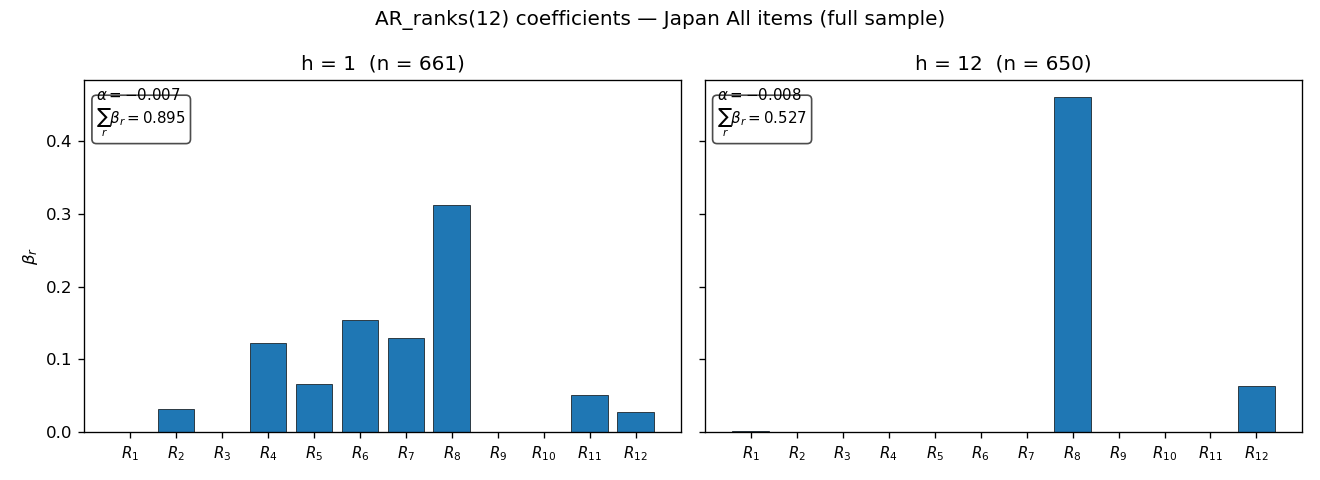
\includegraphics[width=0.95\linewidth]{AR/plots/coef_bars.png}
  \caption{AR\textsubscript{ranks}(12) coefficients, Japan headline CPI,
           full-sample fit. Left: $h\!=\!1$. Right: $h\!=\!12$.}
  \label{fig:ar_ranks_coefs}
\end{figure}

\paragraph{Robustness.}
Three checks are reported in detail in the supplementary materials.
(i) \emph{Subsample stability}: refitting AR\textsubscript{ranks} separately
on the deflation (1995--2012) and post-Abenomics (2013--2025) samples shows
that the $R_8$ concentration is a feature of the deflation regime; the
post-Abenomics fit shifts weight toward higher ranks, consistent with the
return of persistent positive inflation.
(ii) \emph{Consumption-tax dummies}: comparing the raw fit, a fit with
$\pi_t$ masked to \textsc{nan} at the 1997-04, 2014-04, and 2019-10
impact months, and a fit with log-linear interpolation through those months
leaves the coefficient on $R_8$ qualitatively unchanged, but the interpolated
variant redistributes a non-trivial share of weight from $R_8$ to $R_5$ and
$R_{11}$, indicating that tax spikes do influence specific rank loadings
without changing the headline finding.
(iii) \emph{Series choice}: re-running the full table on the
\textit{All items, less fresh food} core series
(Table~\ref{tab:ar_horizon_corecpi}) yields nearly identical patterns to the
headline table, confirming that fresh-food noise is not driving the result.

\begin{table}[htbp]
\centering
\caption{Forecasting Performance: AR family on Japan All items, less fresh food (core)}
\label{tab:ar_horizon_corecpi}
\begin{tabular}{lcccccccccc}
\toprule
 & \multicolumn{5}{c}{Window A (2010m1--2019m12)} & \multicolumn{5}{c}{Window B (2020m1--2025m12)} \\
\cmidrule(lr){2-6} \cmidrule(lr){7-11}
$h \to$ & 1 & 3 & 6 & 12 & 24 & 1 & 3 & 6 & 12 & 24 \\
\midrule
$\text{AR}_{\text{lags}}(12)$     & 1.09 & 0.92 & 0.86 & \textbf{0.79} & 0.66 & 1.42 & 1.18 & 1.23 & 1.32 & 1.23 \\
$\text{AR}^{+}_{\text{lags}}(12)$ & 1.08 & \textbf{0.92} & \textbf{0.86} & 0.79 & 0.67 & 1.41 & 1.18 & 1.22 & 1.31 & \textbf{1.15} \\
$\text{AR}_{\text{ranks}}(12)$    & 1.38 & 1.02 & 0.94 & 0.81 & 0.69 & 1.52 & 1.23 & \textbf{1.16} & \textbf{1.10} & 1.19 \\
AR(1) on YoY                      & \textbf{1.00} & 1.00 & 0.97 & 0.80 & \textbf{0.66} & \textbf{1.01} & \textbf{1.05} & 1.17 & 1.31 & 1.25 \\
\bottomrule
\end{tabular}
\begin{tablenotes}\footnotesize
\item RMSE relative to the random-walk forecast
($\hat{y}^{\text{RW}}_{t+h} = $ current 12-month YoY at $t$, $=1.00$ by
construction, omitted). Column minimum bolded. Expanding-window OOS,
training start 1995-01.
\end{tablenotes}
\end{table}
